\documentclass{article}
\usepackage{enumitem}
\usepackage{algorithm}
\usepackage{algpseudocode}
\usepackage{graphicx}
\begin{document}

%%%%%%%%%%%%%%%%%%%%%%%%%%%%%%%%%%%%%%%%%%%%%%%%%%%%%%%%%%%%%%%%%%%%%
\noindent
\rule{\textwidth}{1pt}
\begin{center}
{\bf [MA202] Numerical Techniques}
\end{center}
Course Instructor: Ashish Phophalia 
\hfill Final Project report \\
\hfill Group Members:
    \item RANISH ABHIJIT JAMODE (202251107)
    \item GAURAV JANARDAN BARHATE (202251049)
    \item ABBAS MULLA ABDUL TAYYAB HAKIMI   (202251002)
    \item PRATIK SINDHIYA (20225103)
\\
\rule{\textwidth}{1pt}
%%%%%%%%%%%%%%%%%%%%%%%%%%%%%%%%%%%%%%%%%%%%%%%%%%%%%%%%%%%


\begin{center}
{\LARGE \textbf{Computational Physics Simulation:}} \\[8pt]
{\LARGE \textbf{Exploring Numerical Integration}}
\end{center}


\subsection*{}


\subsection*{Introduction:}
Our project utilizes numerical integration to simulate physical systems accurately, 
providing insights into real-world phenomena. In our project, we apply the Runge-Kutta method to solve the complex dynamics of the two-body problem. This fundamental problem in celestial mechanics is the gravitational interaction of two enormous masses under Newton's law. For such systems, analytical solutions are not always found, hence accurate simulations require the use of numerical techniques. In order to solve ordinary differential equations, we resort to the time-tested Runge-Kutta method, which is well-known for its precision and adaptability. This technique, which dates back to the late 1800s, offers a reliable foundation for estimating differential equation solutions in a variety of fields.

\subsection*{Components}


In this project, we have developed two applications for simulating the motion of two celestial bodies interacting under the influence of gravity. The first application is implemented in C, while the second one is written in Python. Both applications aim to achieve functional equivalence and consist of separate components for modeling, controlling the simulation, and visualizing the results.


\subsubsection*{Model}

The model component consists of a C structure and a Python class (or data class) named \texttt{TwoBodyModel}. This component stores the necessary data needed to visualize the calculations, such as the positions, velocities, mass ratio, and eccentricity of the two bodies.

\subsubsection*{Controller}

The controller component includes a C structure and a Python class named \texttt{TwoBodyController}. This component stores parameters such as eccentricity, mass ratio, and simulation details. It also contains functions/methods to perform the simulation by numerically solving the related ordinary differential equations using Euler's method or the fourth-order Runge-Kutta method.

\subsubsection*{App}

The app component provides a simple command-line interface allowing users to specify simulation parameters such as the total time (\(T\)), time step (\(Δt\)), mass ratio, eccentricity, and simulation method (e.g., Euler's method or Runge-Kutta). It runs the simulation from \(0\) to \(T\) in steps of \(Δt\) using the \texttt{TwoBodyModel} and \texttt{TwoBodyController}, then saves the location vectors in a text file named \texttt{AnalysisResult.txt}.

\subsubsection*{Animation}

The animation application consists of a single source file written in Python named \texttt{plot\_simulation.py}. It is completely independent of the simulation part and includes the following components:

\subsubsubsection*{View}

The view component is represented by a class named \texttt{TwoBodyView}, which utilizes Tkinter, a built-in GUI toolkit, to draw the two bodies on a window interactively.

\subsubsubsection*{App}

The app component reads the \texttt{AnalysisResult.txt} file generated in the simulation step and visualizes the data using the \texttt{TwoBodyView} class.

\subsection*{Conclusion}

By dividing the project into these components, we achieve modularity and maintainability, allowing for easier development, testing, and debugging. Additionally, the separation of concerns ensures that each component focuses on a specific aspect of the application, promoting code reusability and scalability.


\subsection*{Features:}
\begin{itemize}[label=-]
    \item Numerical Integration Techniques: Utilizes various numerical integration methods to accurately simulate physical systems.
    \item Flexible Simulation Parameters: Allows users to adjust simulation parameters such as time step size and integration method for customized simulations.
    \item Real-time Visualization: Provides real-time visualization of simulated trajectories and physical properties for interactive exploration.
\end{itemize}

\subsection*{Motivation:}
The motivation behind incorporating numerical integration techniques into physics simulation arises from the need to model and understand complex physical phenomena. Many real-world systems, such as celestial mechanics, fluid dynamics, and quantum mechanics, lack analytical solutions and require numerical approaches for accurate prediction. By employing numerical integration, physicists and engineers can gain insights into the behavior of these systems and make informed decisions about design, optimization, and analysis.


\subsection*{Coordinate System}

A surprising fact about the motion of two bodies is that their common center of mass remains still (or moves at constant velocity). We can take advantage of this fact and place the origin of the coordinate system at the center of mass (Figure \ref{fig:coordinate_system}).
  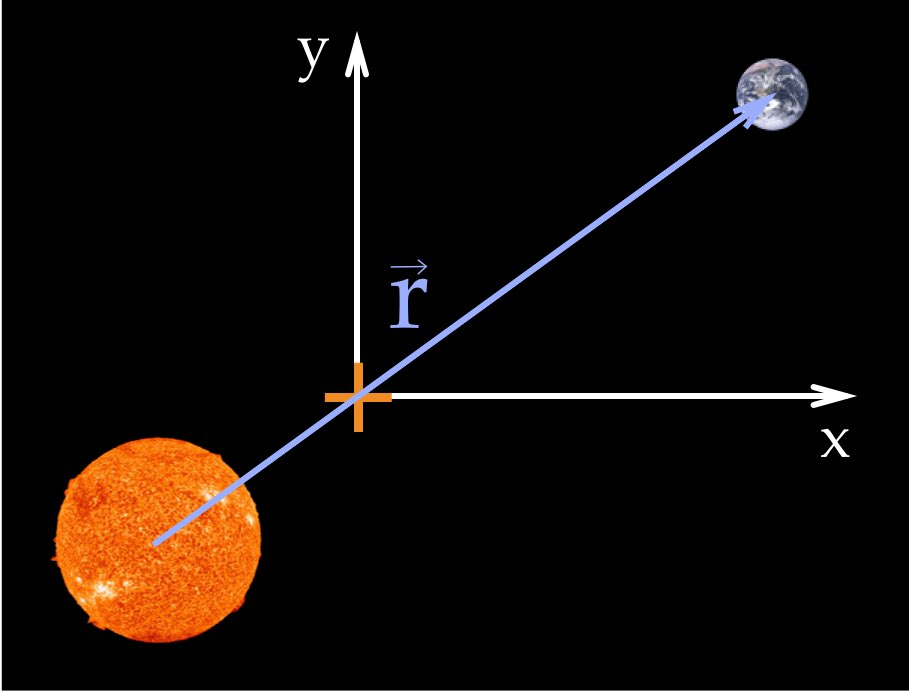
\includegraphics[width=0.5\linewidth]{0010_coordinate_system.jpg}
\begin{figure}
       \caption
        {A coordinate system with the origin at the common center of mass of the two bodies.}
        
        
        
    \label{fig:coordinate_system}
\end{figure}

\subsection*{Newton's Law of Gravitation}

The main equation used in our simulation is Newton’s law of universal gravitation (Equation \ref{eq:newton_gravitation}). It states that the force of gravitational attraction between two bodies is proportional to the product of their masses and inversely proportional to the square of the distance between them.

\begin{equation}
    F = G \frac{{m_1 \cdot m_2}}{{r^2}}
    \label{eq:newton_gravitation}
\end{equation}

Where:
\begin{itemize}
    \item $F$ is the gravitational force between the two bodies,
    \item $G$ is the gravitational constant ($6.674 \times 10^{-11} \, \text{m}^3 \, \text{kg}^{-1} \, \text{s}^{-2}$),
    \item $m_1$ and $m_2$ are the masses of the two bodies,
    \item $r$ is the distance between the centers of the two bodies.
\end{itemize}
\subsection*{Equation of Motion}

After a series of algebraic manipulations and removing dimensions, we can turn Equation \ref{eq:newton_gravitation} into an equation of motion of two bodies, as shown in Equation \ref{eq:equation_motion}. Here, vector $\mathbf{r}$ describes the position of the second body relative to the first one. This vector is depicted as the blue arrow in Figure \ref{fig:coordinate_system}.

\begin{equation}
    \ddot{\mathbf{r}} = -\frac{{(1 + q)}}{{|\mathbf{r}|^3}} \mathbf{r}
    \label{eq:equation_motion}
\end{equation}

The variable $q$ in Equation \ref{eq:equation_motion} represents the mass ratio of the bodies (i.e., the mass of the Earth divided by the Sun’s mass). The two dots above vector $\mathbf{r}$ denote the second time derivative.

\subsection*{Equations of Motion for \(x\) and \(y\)}

Next, we express Equation \ref{eq:equation_motion} in terms of \(x\) and \(y\) coordinates, resulting in a system of two second-order non-linear differential equations:

\begin{align}
    \ddot{x} &= -\frac{{(1 + q)}}{{r^3}} x \\
    \ddot{y} &= -\frac{{(1 + q)}}{{r^3}} y
    \label{eq:equation_motion_xy}
\end{align}

Where:
\begin{itemize}
    \item \(\ddot{x}\) and \(\ddot{y}\) represent the second derivatives of \(x\) and \(y\) with respect to time, respectively,
    \item \(r\) is the distance between the two bodies.
\end{itemize}

\subsection*{Reducing the Order of ODEs}

To solve Equation \ref{eq:equation_motion_xy} numerically, we translate it into a system of first-order ordinary differential equations (ODEs) by making the following substitutions:

\begin{align}
    u_1 &= x \\
    u_2 &= \dot{x} \\
    u_3 &= y \\
    u_4 &= \dot{y}
\end{align}
Equation \ref{eq:equation_motion_xy} can then be expressed as a system of four first-order ODEs:

\begin{align}
    \dot{u}_1 &= u_2 \\
    \dot{u}_2 &= -\frac{{(1 + q)}}{{r^3}} u_1 \\
    \dot{u}_3 &= u_4 \\
    \dot{u}_4 &= -\frac{{(1 + q)}}{{r^3}} u_3
    \label{eq:first_order_odes}
\end{align}

\subsection*{Solving ODEs Numerically}

Now we can utilize a numerical method to solve the ODEs. Instead of Euler’s method, we will employ another popular method called Runge-Kutta:

\begin{verbatim}
double timestep = 0.15;
rungeKutta.calculate(timestep, state.u, derivative);
\end{verbatim}

This code will be executed at each frame of the animation, updating the positions and velocities of the bodies. The first two elements of the \texttt{state.u} array represent the \(x\) and \(y\) positions of the vector \(\mathbf{r}\) from Figure \ref{fig:coordinate_system}. 

\subsubsection*{Runge-Kutta Method}

The Runge-Kutta method is a numerical integration technique used to solve ordinary differential equations. In our implementation, we have the following function:

\begin{verbatim}
void Runge_kutta_calculate(TwoBodyController *this, double h) {
    // coefficients
    double a[4] = {h / 2, h / 2, h, 0};
    double b[4] = {h / 6, h / 3, h / 3, h / 6};
    // arrays for intermediate results
    double u0[4];
    double ut[4];
    double *du;

    // Initialize arrays
    for (int i = 0; i < 4; i++) {
        u0[i] = this->model->u[i];
        ut[i] = 0;
    }

    // Runge-Kutta iteration
    for (int j = 0; j < 4; j++) {
        du = derivative(this);
        for (int i = 0; i < 4; i++) {
            this->model->u[i] = u0[i] + a[j] * du[i];
            ut[i] = ut[i] + b[j] * du[i];
        }
    }

    // Update final results
    for (int i = 0; i < 4; ++i)
        this->model->u[i] = u0[i] + ut[i];

    free(du); // Free dynamically allocated memory
}
\end{verbatim}

This function calculates the new state of the system using the Runge-Kutta method with a given timestep (\(h\)). The derivative function is called to compute the derivative of the state variables.

\newpage
\subsection*{Drawing Two Bodies on the Screen}

Now that we have determined the vector $\mathbf{r}$, which describes the position of Earth relative to the Sun, we can use this information to calculate the positions of the two bodies on the screen. We utilize the mass-distance relation depicted in Figure \ref{fig:mass_distance}.

With this knowledge, we can calculate the positions of the two bodies. The positions are stored in the \texttt{state.positions} array and then used to display the two bodies on the screen.

\subsubsection*{Implementation}

We can incorporate the calculation of body positions into the animation loop. Below is a simplified version of the code:

\begin{verbatim}
void calculate_new_position(TwoBodyController *this) {
    double r = 1.0; // Assuming a distance of 1 unit for simplicity
    double a1 = (this->model->mass2 / this->model->mass12) * r;
    double a2 = (this->model->mass1 / this->model->mass12) * r;

    // Calculate positions of the bodies
    this->model->Planet1.x = -a2 * this->model->u[0];
    this->model->Planet1.y = -a2 * this->model->u[1];
    this->model->Planet2.x = a1 * this->model->u[0];
    this->model->Planet2.y = a1 * this->model->u[1];
}
\end{verbatim}

In this function, we calculate the positions of the two bodies based on the mass-distance relation. The positions are then assigned to the respective body objects, which can be used for rendering.

\begin{figure}[b]
    \centering
    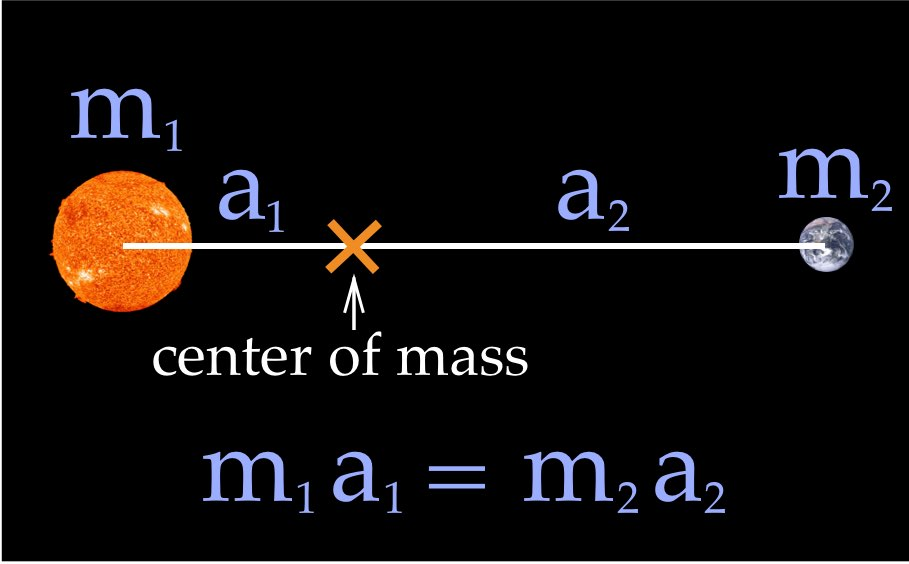
\includegraphics[width=0.5\linewidth]{mass_distance_relation.jpg}
    \caption{A relation between masses of two bodies and distances to the common center of mass.}
    \label{fig:mass_distance}
\end{figure}

\newpage
\subsection*{How it Works:}
The physics simulation framework operates by discretizing the equations of motion governing the system and applying numerical integration methods to approximate the continuous evolution of the system over time. Users specify initial conditions, physical parameters, and integration settings, and the framework computes the system's trajectory and properties through numerical integration. Real-time visualization tools allow users to observe the simulated system's behavior and analyze its dynamics.
\subsection*{Project Structure:}
The project consists of multiple components responsible for numerical integration, simulation control, and visualization:

\begin{itemize}[label=-]
    \item Numerical Integration Modules:
    \begin{itemize}[label=$\bullet$]
        \item \texttt{Euler Method}: Implements the basic Euler method for numerical integration.
        \item \texttt{Runge-Kutta Methods}: Includes higher-order Runge-Kutta methods such as the fourth-order method.
        \item \texttt{Adaptive Integration}: Implements adaptive integration techniques to dynamically adjust the time step size.
    \end{itemize}
    
    \item Simulation Control:
    \begin{itemize}[label=$\bullet$]
        \item \texttt{Simulation Parameters}: Provides functionality for specifying initial conditions, physical parameters, and integration settings.
        \item \texttt{Time Stepping}: Controls the advancement of simulation time and iteration over time steps.
    \end{itemize}
    
    \item Visualization Components:
    \begin{itemize}[label=$\bullet$]
        \item \texttt{Graphics Interface}: Utilizes the Tkinter library to create a graphical user interface (GUI) for real-time visualization.
        \item \texttt{Data Reading}: Reads simulation data from files generated during simulation runs.
        \item \texttt{Animation}: Animates the trajectories of simulated bodies using graphical elements such as ovals and lines.
    \end{itemize}
\end{itemize}
\newpage
\subsection*{Implementation:}
The project implementation includes the integration of numerical methods, simulation control logic, and visualization components:

\begin{itemize}[label=-]
    \item \texttt{Numerical Integration Modules}: Each numerical integration method is implemented as a separate module, providing flexibility and choice for simulation accuracy and efficiency.
    \item \texttt{Simulation Control}: Functionalities for initializing simulation parameters, controlling simulation execution, and managing time stepping are implemented to ensure accurate and efficient simulation runs.
    \item \texttt{Visualization Components}: The graphical user interface (GUI) developed using Tkinter allows users to interact with the simulation in real-time. Simulation data is read from files generated during simulation runs, and the animation module animates the trajectories of simulated bodies using graphical elements.
\end{itemize}

\subsection*{Additional Visualization Component:}
The provided code includes a Python script utilizing Tkinter for real-time visualization of the two-body simulation. This component enhances the project by providing a graphical representation of the simulated trajectories, allowing users to visually observe the dynamics of the system.





\subsection*{Implementation:}
Each numerical integration method is implemented as a separate module within the project, providing users with flexibility and choice based on their simulation requirements. The framework offers a user-friendly interface for specifying system parameters, integration settings, and visualization preferences. By leveraging numerical integration techniques, the framework enables researchers, educators, and engineers to explore and analyze diverse physical systems with precision and insight.

\subsubsection*{Explanation of the Code:two_body_simulation.c}

\textbf{Constants and Libraries:}
The code includes necessary libraries (\texttt{stdio.h}, \texttt{stdlib.h}, \texttt{math.h}) and declares global constants for initial eccentricity and $q$ values.

\textbf{Data Structures:}
Two structures are defined: \texttt{Body}, representing a celestial body's position, and \texttt{TwoBodyModel}, representing the two-body system's state.

\textbf{Function Pointers and Views:}
The code introduces function pointers and a view structure (\texttt{TwoBodyView}) for displaying simulation results.

\textbf{Controller Structure and Initialization:}
A controller structure (\texttt{TwoBodyController}) is defined to manage the simulation process. It includes pointers to the model and view components.

\textbf{Display Function and Console View:}
The \texttt{console\_display()} function writes simulation data to a file. The \texttt{create\_console\_view()} function initializes a console view for displaying simulation results.

\textbf{Initial Velocity Calculation:}
The \texttt{initialVelocity()} function computes the initial velocity of the two bodies based on the given eccentricity and $q$ values.

\textbf{Resetting Initial Conditions:}
The \texttt{reset\_state\_to\_initial\_conditions()} function initializes the simulation by setting initial conditions for the two bodies, including positions, velocities, and masses.

\textbf{Derivative Calculation:}
The \texttt{derivative()} function computes the derivatives of the state variables (position and velocity) using the current state of the system. It is used in numerical integration algorithms.

\textbf{Runge-Kutta Integration:}
The \texttt{Runge\_kutta\_calculate()} function performs Runge-Kutta integration to update the system's state over a given time step. It iteratively calculates intermediate values to approximate the solution.

\textbf{Calculating New Positions:}
The \texttt{calculate\_new\_position()} function updates the positions of the two bodies based on the current state of the system.

\textbf{Main Function and Simulation Loop:}
The \texttt{main()} function initializes the simulation, including file handling, model setup, and view initialization. It then iterates over a fixed number of time steps, updating the system's state and displaying results.

\textbf{Closing File:}
Finally, the code closes the file used for storing simulation results.

\subsection*{Overall:}
\begin{itemize}[label=-]
    \item This code provides a framework for simulating the dynamics of a two-body system using numerical integration techniques.
    \item It encapsulates the simulation logic into distinct modules, facilitating code organization and maintainability.
\end{itemize}

\begin{algorithm}
\caption{Console Display}
\begin{algorithmic}[1]
\Function{console\_display}{$\text{this}$}
    \State Write $\text{this} \rightarrow \text{model} \rightarrow \text{Planet1.x}$, $\text{this} \rightarrow \text{model} \rightarrow \text{Planet1.y}$, $\text{this} \rightarrow \text{model} \rightarrow \text{Planet2.x}$, $\text{this} \rightarrow \text{model} \rightarrow \text{Planet2.y}$ to file
\EndFunction
\end{algorithmic}
\end{algorithm}

\begin{algorithm}
\caption{Create Console View}
\begin{algorithmic}[1]
\Function{create\_console\_view}{$\text{this}$}
    \State Set $\text{this} \rightarrow \text{display}$ to $\text{console\_display}$
\EndFunction
\end{algorithmic}
\end{algorithm}

\begin{algorithm}
\caption{Reset State to Initial Conditions}
\begin{algorithmic}[1]
\Function{reset\_state\_to\_initial\_conditions}{$\text{this}$}
    \State Set $\text{this} \rightarrow \text{model} \rightarrow q$ to $\text{initial\_q}$
    \State Set $\text{this} \rightarrow \text{model} \rightarrow \text{eccentricity}$ to $\text{initial\_eccentricity}$
    \State Set $\text{this} \rightarrow \text{model} \rightarrow u[0]$ to $1.0$
    \State Set $\text{this} \rightarrow \text{model} \rightarrow u[1]$ to $0.0$
    \State Set $\text{this} \rightarrow \text{model} \rightarrow u[2]$ to $0.0$
    \State Set $\text{this} \rightarrow \text{model} \rightarrow u[3]$ to $\text{initialVelocity}(\text{this} \rightarrow \text{model} \rightarrow q, \text{this} \rightarrow \text{model} \rightarrow \text{eccentricity})$
    \State Set $\text{this} \rightarrow \text{model} \rightarrow \text{mass1}$ to $1.0$
    \State Set $\text{this} \rightarrow \text{model} \rightarrow \text{mass2}$ to $\text{this} \rightarrow \text{model} \rightarrow q$
    \State Set $\text{this} \rightarrow \text{model} \rightarrow \text{mass12}$ to $\text{this} \rightarrow \text{model} \rightarrow \text{mass1} + \text{this} \rightarrow \text{model} \rightarrow \text{mass2}$
    \State Set $\text{this} \rightarrow \text{model} \rightarrow \text{Planet1.x}$ to $0$
    \State Set $\text{this} \rightarrow \text{model} \rightarrow \text{Planet2.x}$ to $0$
    \State Set $\text{this} \rightarrow \text{model} \rightarrow \text{Planet1.y}$ to $0$
    \State Set $\text{this} \rightarrow \text{model} \rightarrow \text{Planet2.y}$ to $0$
\EndFunction
\end{algorithmic}
\end{algorithm}

\begin{algorithm}
\caption{Derivative Calculation}
\begin{algorithmic}[1]
\Function{derivative}{$\text{this}$}
    \State Allocate memory for array $\text{du}[4]$
    \State Calculate $r[2]$ as $\text{this} \rightarrow \text{model} \rightarrow u[0]$, $\text{this} \rightarrow \text{model} \rightarrow u[1]$
    \State Calculate $\text{rr}$ as $\sqrt{r[0]^2 + r[1]^2}$
    \For{$i$ \textbf{from} $0$ \textbf{to} $1$}
        \State Set $\text{du}[i]$ to $\text{this} \rightarrow \text{model} \rightarrow u[i + 2]$
        \State Set $\text{du}[i + 2]$ to $-(1 + \text{this} \rightarrow \text{model} \rightarrow q) \times r[i] / \text{pow}(\text{rr}, 3)$
    \EndFor
    \State \textbf{return} $\text{du}$
\EndFunction
\end{algorithmic}
\end{algorithm}

\begin{algorithm}
\caption{Runge-Kutta Integration Calculation}
\begin{algorithmic}[1]
\Function{Runge\_kutta\_calculate}{$\text{this}, h$}
    \State Initialize arrays $a[4]$, $b[4]$, $u0[4]$, $ut[4]$ with appropriate values
    \For{$j$ \textbf{from} $0$ \textbf{to} $3$}
        \State $du \gets \text{derivative}(\text{this})$
        \For{$i$ \textbf{from} $0$ \textbf{to} $3$}
            \State Update state variables: $\text{this} \rightarrow \text{model} \rightarrow u[i] \gets u0[i] + a[j] \times du[i]$
            \State Update intermediate values: $ut[i] \gets ut[i] + b[j] \times du[i]$
        \EndFor
    \EndFor
    \For{$i$ \textbf{from} $0$ \textbf{to} $3$}
        \State Update state variables: $\text{this} \rightarrow \text{model} \rightarrow u[i] \gets u0[i] + ut[i]$
    \EndFor
    \State Free dynamically allocated memory
\EndFunction
\end{algorithmic}
\end{algorithm}

\begin{algorithm}
\caption{Update Position}
\begin{algorithmic}[1]
\Function{update\_position}{$\text{this}$}
    \State Set $\text{timestep}$ to $0.15$
    \State Call \textsc{Runge\_kutta\_calculate}($\text{this}, \text{timestep}$)
    \State Call \textsc{calculate\_new\_position}($\text{this}$)
\EndFunction
\end{algorithmic}
\end{algorithm}

\begin{algorithm}
\caption{Main Function}
\begin{algorithmic}[1]
\Function{main}{}
    \State Open file $\text{AnalysisResult.txt}$ for writing
    \State Declare variables $\text{planet1}$, $\text{planet2}$, $\text{model}$, $\text{view}$, $\text{controller}$
    \State Initialize $\text{controller} \rightarrow \text{model}$ with $\text{planet1}$, $\text{planet2}$
    \State Initialize $\text{controller} \rightarrow \text{view}$
    \State Call \textsc{create\_console\_view}($\text{view}$)
    \State Call \textsc{reset\_state\_to\_initial\_conditions}($\text{controller}$)
    \For{$i$ \textbf{from} $0$ \textbf{to} $999$}
        \State Call \textsc{update\_position}($\text{controller}$)
        \State Call $\text{controller} \rightarrow \text{view} \rightarrow \text{display}(\text{controller} \rightarrow \text{model})$
    \EndFor
    \State Close file
\EndFunction
\end{algorithmic}
\end{algorithm}

\newpage
\subsubsection*{Explanation of the Code: \texttt{plot\_simulation.py}}

\textbf{Imports and Libraries:}
The script begins by importing the necessary libraries: \texttt{time} for timing purposes and \texttt{tkinter} for creating the graphical user interface (GUI).

\textbf{View Class Definition:}
A class named \texttt{TwoBodyView} is defined to manage the GUI for visualizing the simulation results. It initializes the GUI window, canvas, and sets up the initial positions of the celestial bodies.

\textbf{Data Reading:}
The \texttt{read\_data()} method within the \texttt{TwoBodyView} class reads data from the file \texttt{AnalysisResult.txt}. It parses the data and stores it in a list for animation.

\textbf{GUI Setup:}
The \texttt{setup\_gui()} method configures the Tkinter window, canvas, and positions the two celestial bodies (represented as circles) on the canvas.

\textbf{Animation:}
The \texttt{animate()} method within the \texttt{TwoBodyView} class iterates through the data obtained from the file. It updates the positions of the celestial bodies on the canvas based on the data points and creates lines to trace their movement.

\textbf{Main Execution:}
An instance of the \texttt{TwoBodyView} class is created, which initializes the GUI and starts the animation loop. The \texttt{mainloop()} function of Tkinter is called to display the GUI and animate the celestial bodies.

\subsection*{Overall:}
\begin{itemize}[label=-]
    \item This Python script provides a simple and interactive way to visualize the simulation results of the two-body system.
    \item It leverages Tkinter for GUI creation and animation, making it accessible and user-friendly.
\end{itemize}

\begin{algorithm}
\caption{Read Data}
\begin{algorithmic}[1]
\Function{read\_data}{}
    \State Open file \texttt{AnalysisResult.txt}
    \For{each line \textbf{in} file}
        \State Split line by comma and store in \texttt{x}
        \State Append \texttt{x} to \texttt{empty\_list}
    \EndFor
\EndFunction
\end{algorithmic}
\end{algorithm}

\begin{algorithm}
\caption{Animate}
\begin{algorithmic}[1]
\Function{animate}{$i$}
    \If{$i < $ length of \texttt{empty\_list}}
        \State Move \texttt{planet\_one} by calculated distance
        \State Move \texttt{planet\_two} by calculated distance
        \State Create line for \texttt{planet\_one} with color red
        \State Create line for \texttt{planet\_two} with color blue
        \State Update GUI
        \State Sleep for 0.00001 seconds
        \State Schedule next animation frame
    \EndIf
\EndFunction
\end{algorithmic}
\end{algorithm}
\clearpage
\vspace*{\fill}
\begin{center}
    \subsection*{\huge Final Results and Simulation}
\end{center}
\vspace*{\fill}


\begin{figure}[htbp]

    \centering
    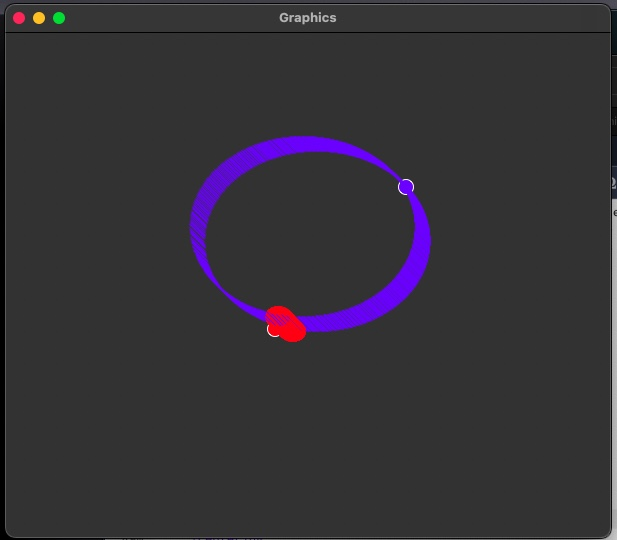
\includegraphics[width=0.5\linewidth]{Image 20-04-24 at 10.31 PM.jpg}
    
    \caption{Final Simulation}
    \label{fig:final-simulation}

    \centering
    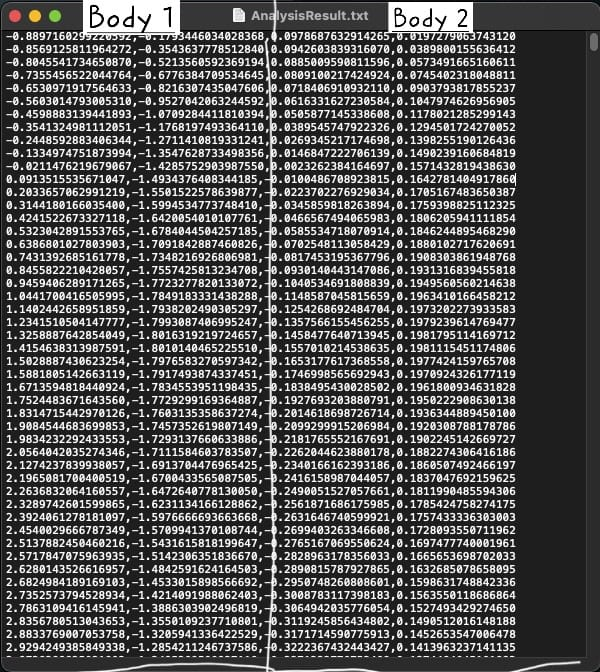
\includegraphics[width=0.5\linewidth]{WhatsApp Image 2024-04-20 at 22.24.56 (1).jpeg}
    \caption{Body one and Body 2 coordinates}
    \label{fig:enter-label}
\end{figure}
\vspace*{\fill}
\begin{center}
\subsection*{\large Thank You}
\end{center}
\vspace*{\fill}
\end{document}